%%%%%%%%%%%%%%%%%%%%%%%%%%%%%%%%%%%%%%%%%
% Short Sectioned Assignment
% LaTeX Template
% Version 1.0 (5/5/12)
%
% This template has been downloaded from:
% http://www.LaTeXTemplates.com
%
% Original author:
% Frits Wenneker (http://www.howtotex.com)
%
% License:
% CC BY-NC-SA 3.0 (http://creativecommons.org/licenses/by-nc-sa/3.0/)
%
%%%%%%%%%%%%%%%%%%%%%%%%%%%%%%%%%%%%%%%%%

%----------------------------------------------------------------------------------------
%	PACKAGES AND OTHER DOCUMENT CONFIGURATIONS
%----------------------------------------------------------------------------------------

\documentclass[paper=a4, fontsize=11pt]{scrartcl} % A4 paper and 11pt font size

\usepackage[T1]{fontenc} % Use 8-bit encoding that has 256 glyphs
\usepackage{fourier} % Use the Adobe Utopia font for the document - comment this line to return to the LaTeX default
\usepackage[english]{babel} % English language/hyphenation
\usepackage{amsmath,amsfonts,amsthm} % Math packages

\usepackage{lipsum} % Used for inserting dummy 'Lorem ipsum' text into the template
\usepackage{graphicx}

\usepackage{sectsty} % Allows customizing section commands
\allsectionsfont{\centering \normalfont\scshape} % Make all sections centered, the default font and small caps

\usepackage{fancyhdr} % Custom headers and footers
\pagestyle{fancyplain} % Makes all pages in the document conform to the custom headers and footers
\fancyhead{} % No page header - if you want one, create it in the same way as the footers below
\fancyfoot[L]{} % Empty left footer
\fancyfoot[C]{} % Empty center footer
\fancyfoot[R]{\thepage} % Page numbering for right footer
\renewcommand{\headrulewidth}{0pt} % Remove header underlines
\renewcommand{\footrulewidth}{0pt} % Remove footer underlines
\setlength{\headheight}{13.6pt} % Customize the height of the header

\numberwithin{equation}{section} % Number equations within sections (i.e. 1.1, 1.2, 2.1, 2.2 instead of 1, 2, 3, 4)
\numberwithin{figure}{section} % Number figures within sections (i.e. 1.1, 1.2, 2.1, 2.2 instead of 1, 2, 3, 4)
\numberwithin{table}{section} % Number tables within sections (i.e. 1.1, 1.2, 2.1, 2.2 instead of 1, 2, 3, 4)

\setlength\parindent{0pt} % Removes all indentation from paragraphs - comment this line for an assignment with lots of text

%----------------------------------------------------------------------------------------
%	TITLE SECTION
%----------------------------------------------------------------------------------------

\newcommand{\horrule}[1]{\rule{\linewidth}{#1}} % Create horizontal rule command with 1 argument of height

\title{	
\normalfont \normalsize 
\textsc{University of Iowa, Professor Omar Haider} \\ [25pt] % Your university, school and/or department name(s)
\horrule{0.5pt} \\[0.4cm] % Thin top horizontal rule
\huge Databases in OpenEMR \\ % The assignment title
\horrule{2pt} \\[0.5cm] % Thick bottom horizontal rule
}

\author{Junhyuk Kang} % Your name

\date{Oct 25, 2016 ~ Nov 1, 2016 } % Today's date or a custom date


\begin{document}

\maketitle % Print the title

%----------------------------------------------------------------------------------------
%	PROBLEM 1
%----------------------------------------------------------------------------------------
\section{Question}
\begin{enumerate}
	\item Validate the hypothesis that the number associated with corresponds to the role of the user who performed the action
	\item Determine how detailed the information in the Log is

\end{enumerate}
%----------------------------------------------------------------------------------------
%	PROBLEM 2
%----------------------------------------------------------------------------------------

\section{Answer Steps}

%------------------------------------------------
\begin{itemize}
	\item I already made multiple users for each roles, so I just used those accounts
	\item I opened same user (5th user) with all different roles
		\begin{itemize}
		\item
		 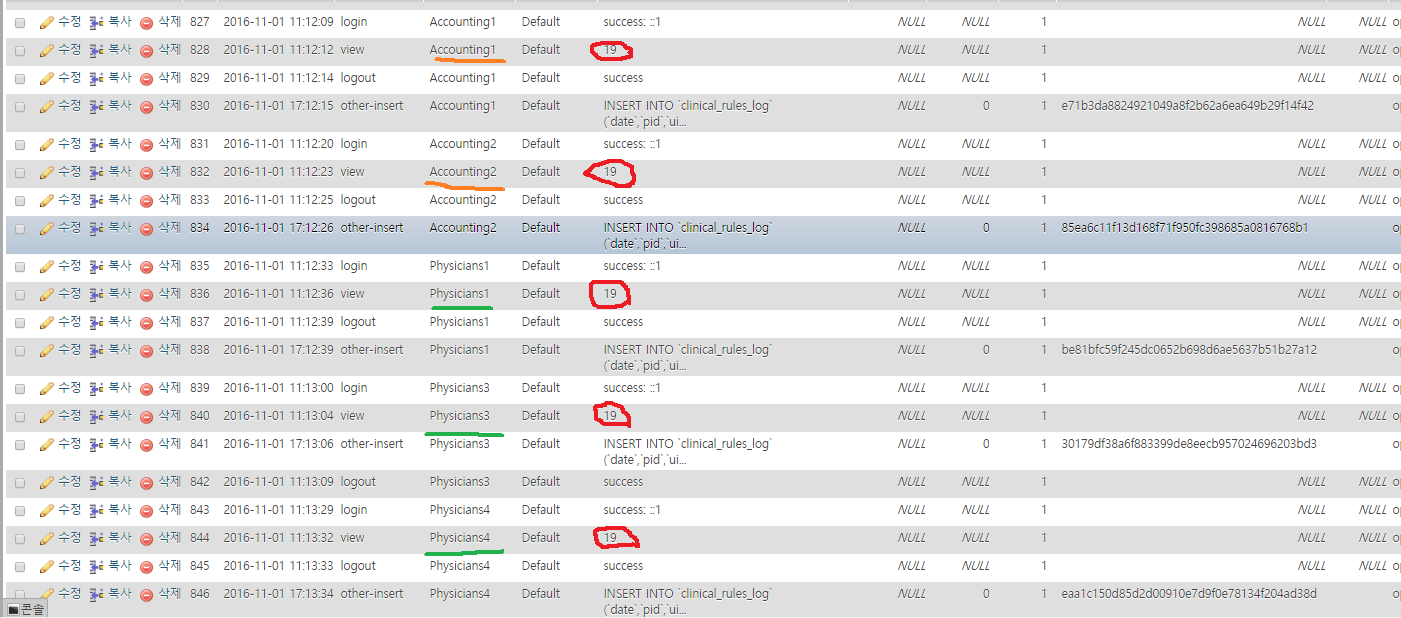
\includegraphics[width = 20cm, height=10cm]{pictures/same19.png}
		\item The log had same number 19 regardless of the user types
		\end{itemize}
	\item I opened same user (3th user) with all different roles again
		\begin{itemize}
		\item
		 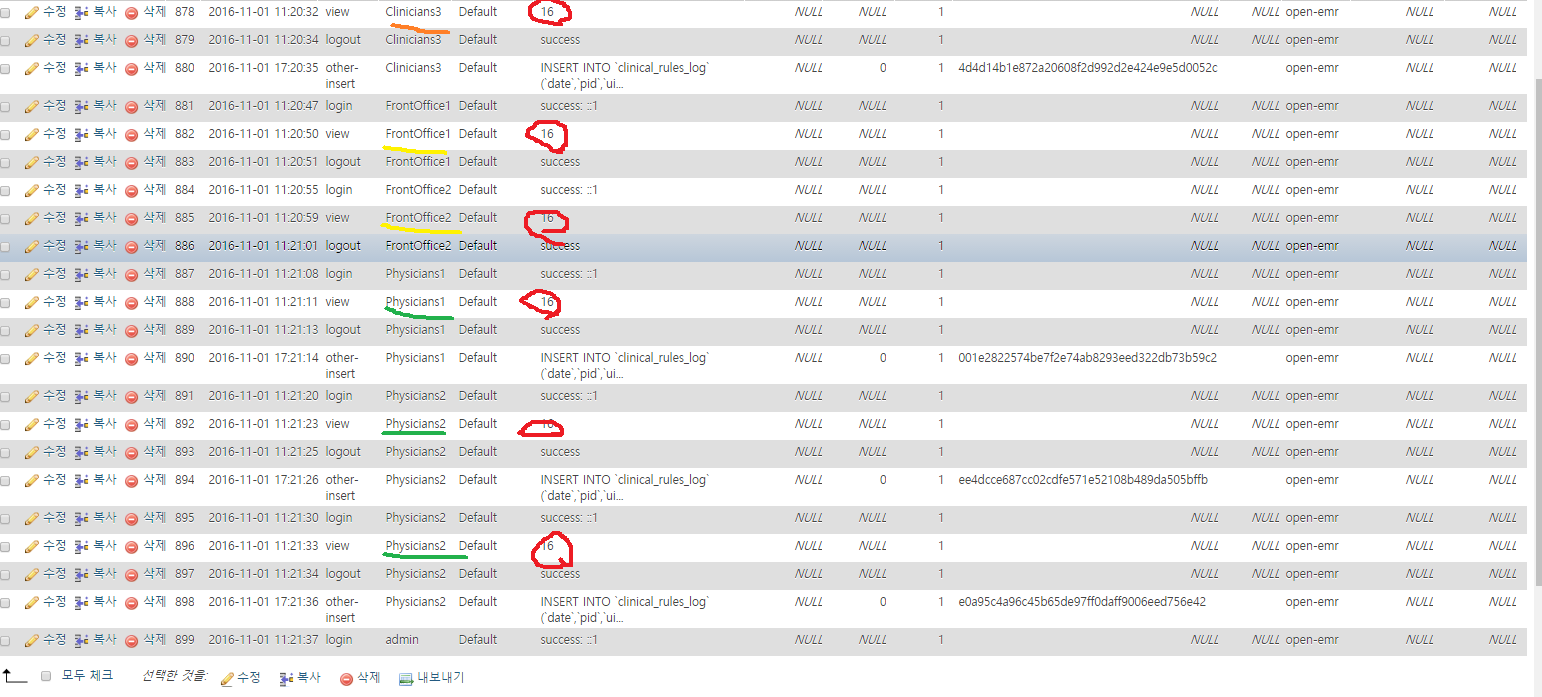
\includegraphics[width = 20cm, height=10cm]{pictures/same16.png}
		\item
		 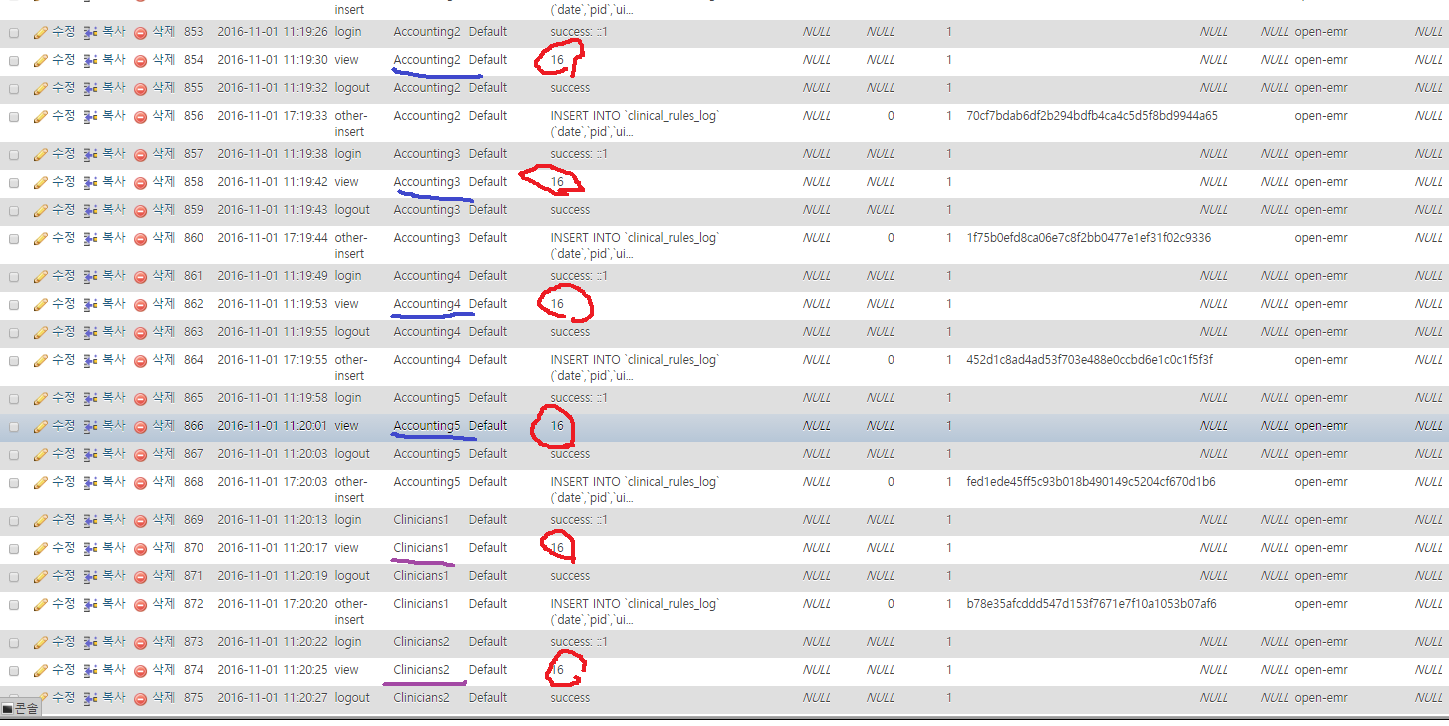
\includegraphics[width = 20cm, height=10cm]{pictures/same162.png}
		\item The log had same number 16 regardless of the user types
		\end{itemize}
	\item In conclusion, number represents the patients regardless of the user types
	\item Then, I tried to find detail logs by doing detail actions other than just opening patient information
		\item Firstly, I copied some word in patient info by clicking right button
		\begin{itemize}
		\item
		 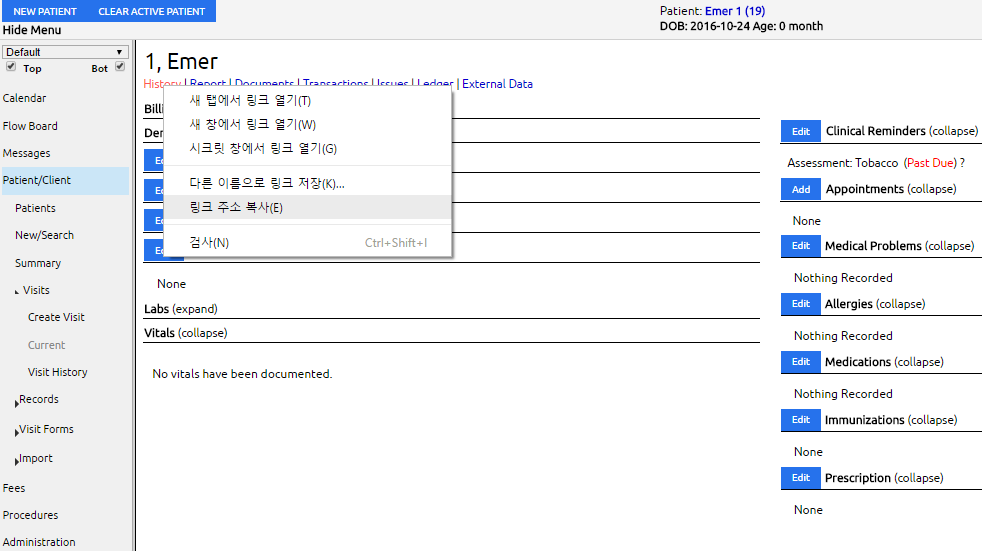
\includegraphics[width = 20cm, height=10cm]{pictures/saving.png}
		\item but log looks same with when I only opened patient info
		\item
		 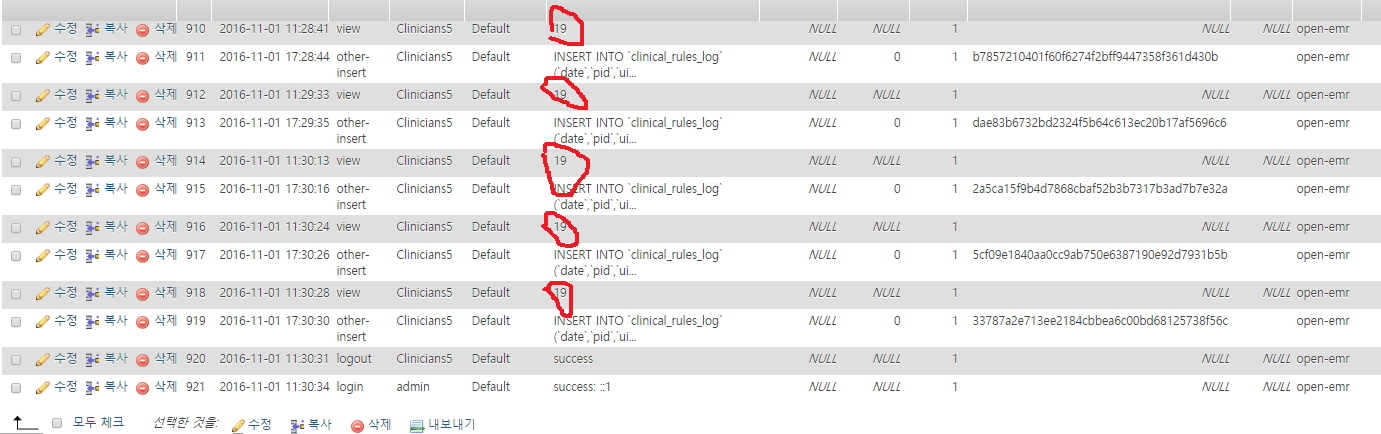
\includegraphics[width = 20cm, height=10cm]{pictures/stillsame.png}
		\item so I copied again some information in patients
		\item
		 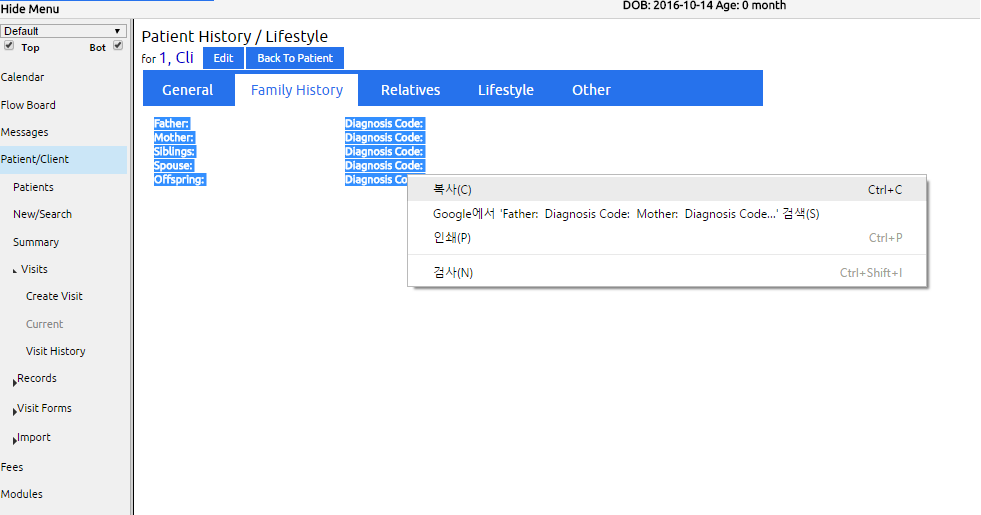
\includegraphics[width = 20cm, height=10cm]{pictures/copyagain.png}
		\item
		 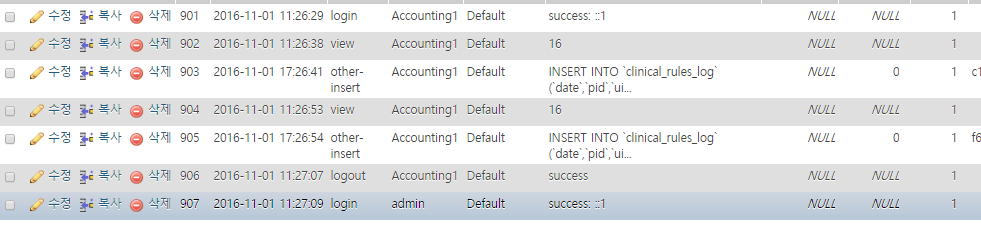
\includegraphics[width = 20cm, height=10cm]{pictures/didntchange.png}
		\item The log was same
\end{itemize}
	\item so I tried to do more actions. (I navigated inside patients file)
		\begin{itemize}
		\item
		 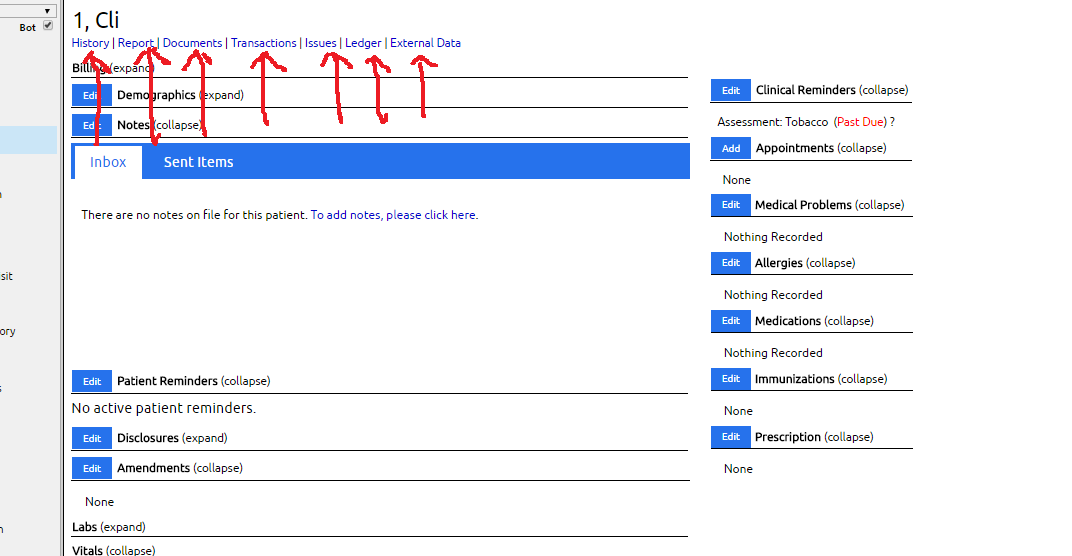
\includegraphics[width = 20cm, height=10cm]{pictures/navigate.png}
		\item
		 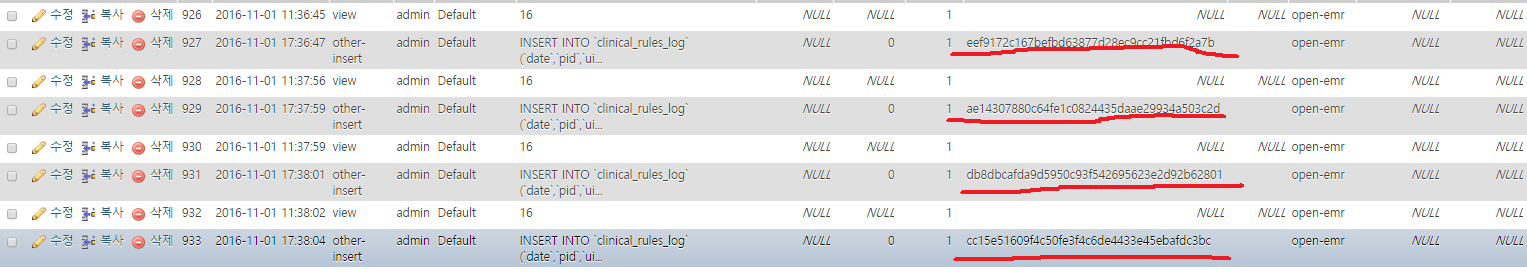
\includegraphics[width = 20cm, height=10cm]{pictures/checksum.png}
		\item Found the difference only in checksum
	\end{itemize}				
\end{itemize}












\end{document}